\documentclass[12pt,a4paper]{article}

\usepackage[utf8]{inputenc}
\usepackage[T1]{fontenc}
\usepackage[brazil]{babel}
\usepackage{lmodern}
\usepackage[a4paper,margin=2.5cm]{geometry}
\usepackage{amsmath,amssymb}
\usepackage{graphicx}
\usepackage{booktabs}
\usepackage{float}
\usepackage{caption}
\usepackage{xcolor}
\usepackage{listings}
\usepackage[hidelinks]{hyperref}

\definecolor{codebg}{RGB}{248,248,248}
\definecolor{codecomment}{RGB}{0,110,0}
\definecolor{codekw}{RGB}{0,0,160}
\definecolor{codestr}{RGB}{160,40,40}

\lstset{
  language=Python,
  basicstyle=\ttfamily\footnotesize,
  backgroundcolor=\color{codebg},
  keywordstyle=\color{codekw}\bfseries,
  commentstyle=\color{codecomment}\itshape,
  stringstyle=\color{codestr},
  numbers=left,
  numberstyle=\tiny\color{gray},
  frame=single,
  breaklines=true,
  showstringspaces=false,
  tabsize=4,
  inputencoding=utf8,
  extendedchars=true,
  literate=
    {á}{{\'a}}1 {à}{{\`a}}1 {ã}{{\~a}}1 {â}{{\^a}}1
    {é}{{\'e}}1 {ê}{{\^e}}1 {í}{{\'i}}1
    {ó}{{\'o}}1 {õ}{{\~o}}1 {ô}{{\^o}}1
    {ú}{{\'u}}1 {ç}{{\c{c}}}1
    {Á}{{\'A}}1 {É}{{\'E}}1 {Í}{{\'I}}1 {Ó}{{\'O}}1 {Ú}{{\'U}}1 {Ç}{{\c{C}}}1
}

% Link do repositório do código
\newcommand{\repositorio}{\url{https://github.com/juliaPamplona/teia-laboratorios/tree/main/lab01}}

\begin{document}

%=====================================================================
% Capa (página 1)
%=====================================================================
\begin{titlepage}
\centering

\includegraphics[width=0.35\textwidth]{figuras/logo_uepb.png}\\[1.5em]
{\large \textsc{Universidade Estadual da Paraíba}}\\[0.3em]
{\normalsize Disciplina: Tópicos Especiais em Inteligência Artificial}\\[0.3em]
{\normalsize Prof. Robson Pequeno de Sousa}

\vfill

{\LARGE \textbf{Classificador de Distância Mínima e Funções de Decisão aplicados à base Iris}}\\[1em]
{\large Relatório do Laboratório 01 --- Reconhecimento com base em decisão teórica}

\vfill

{\large Júlia Pamplona}

\vfill

{\large Setembro de 2026}
\end{titlepage}

%=====================================================================
% Resumo (página 2)
%=====================================================================
\begin{abstract}
Este relatório descreve a implementação, em Python e sem o uso de bibliotecas de aprendizado de máquina, de um sistema de reconhecimento supervisionado de padrões para a base de dados Iris, fundamentado na abordagem de reconhecimento por decisão teórica. Foram implementados (i) o classificador de distância mínima, (ii) o classificador pelo máximo das funções de decisão e (iii) as superfícies de decisão entre pares de classes. Todos os sistemas utilizam o terceiro e o quarto atributos da base, comprimento e largura da pétala. Os dois classificadores obtiveram 93,33\% de acurácia no conjunto de teste, com predições idênticas, o que confirma empiricamente a equivalência teórica entre eles. As retas de decisão separam perfeitamente a classe \emph{setosa} das demais e atingem 94\% de acerto no par \emph{versicolor}~$\times$~\emph{virginica}, cujas nuvens de dados se tocam apenas numa pequena região de fronteira.

\vspace{1em}
\noindent\textbf{Palavras-chave:} reconhecimento de padrões; classificador de distância mínima; funções de decisão; superfície de decisão; base Iris.
\end{abstract}
\thispagestyle{empty}
\newpage

%=====================================================================
% Sumário (página 3)
%=====================================================================
\tableofcontents
\thispagestyle{empty}
\newpage

%=====================================================================
\section{Introdução}
%=====================================================================

O reconhecimento de padrões supervisionado parte do pressuposto de que há um conjunto de treinamento com rótulos conhecidos e de que o classificador é projetado explorando essa informação \emph{a priori}. Entre as técnicas clássicas dessa categoria estão o classificador de distância mínima, o método da máxima verossimilhança e o método de Bayes. Este laboratório trata da primeira delas e de sua formulação equivalente por funções de decisão.

A abordagem por decisão teórica baseia-se em encontrar $W$ funções de decisão (ou funções discriminantes) $d_1(\mathbf{x}), \dots, d_W(\mathbf{x})$ tais que um padrão $\mathbf{x}$ pertence à classe $\omega_i$ se $d_i(\mathbf{x})$ tiver o maior valor numérico entre todas elas.

O objetivo do trabalho é aplicar esses conceitos à base Iris, cumprindo os seguintes requisitos:
\begin{enumerate}
  \item dividir a amostra em 70\% para treinamento e 30\% para teste (a validação fica para um momento posterior);
  \item plotar diagramas de dispersão com os dois primeiros atributos nos cenários \emph{setosa}~$\times$~\emph{versicolor}, \emph{setosa}~$\times$~\emph{virginica} e \emph{versicolor}~$\times$~\emph{virginica};
  \item definir, com os quatro atributos, (i) o classificador de distância mínima e (ii) o classificador de máximo das funções de decisão, ambos para as três classes;
  \item (iii) definir a superfície de decisão (reta) com os dois primeiros atributos para os três cenários e visualizá-la sobre o conjunto de teste e sobre toda a amostra;
  \item não utilizar bibliotecas de aprendizado de máquina.
\end{enumerate}

Neste trabalho, todos os sistemas (classificadores, superfícies de decisão e diagramas de dispersão) foram construídos com o \emph{terceiro e o quarto atributos} da base, isto é, comprimento e largura da pétala. A escolha permite que um único vetor de características bidimensional seja usado de forma consistente nos três métodos, de modo que as retas visualizadas nos gráficos sejam exatamente as fronteiras dos classificadores avaliados. Além disso, essas são as dimensões em que as espécies se diferenciam com mais clareza, conforme discutido na Seção~\ref{sec:discussao}.

%=====================================================================
\section{Fundamentação teórica}\label{sec:teoria}
%=====================================================================

\subsection{Funções de decisão e fronteiras}

Seja $\mathbf{x} = [x_1, x_2, \dots, x_n]^t$ um vetor de características $n$-dimensional associado às classes $\omega_1, \omega_2, \dots, \omega_W$. A regra de decisão é
\begin{equation}
  \mathbf{x} \in \omega_i \quad \text{se} \quad d_i(\mathbf{x}) > d_j(\mathbf{x}), \quad j \neq i = 1, 2, \dots, W.
  \label{eq:regra}
\end{equation}

A fronteira de decisão que separa $\omega_i$ de $\omega_j$ é o lugar geométrico onde as duas funções se igualam:
\begin{equation}
  d_{ij}(\mathbf{x}) = d_i(\mathbf{x}) - d_j(\mathbf{x}) = 0,
  \label{eq:fronteira}
\end{equation}
de modo que $d_{ij}(\mathbf{x}) > 0 \Rightarrow \mathbf{x} \in \omega_i$ e $d_{ij}(\mathbf{x}) < 0 \Rightarrow \mathbf{x} \in \omega_j$.

\subsection{Reconhecimento baseado em casamento: classificador de distância mínima}

No reconhecimento baseado em casamento, cada classe é representada por um vetor protótipo, e um padrão desconhecido é atribuído à classe mais próxima segundo uma métrica predefinida. O caso mais simples é o classificador de distância mínima com distância euclidiana. O protótipo da classe $\omega_j$ é o vetor média de suas amostras:
\begin{equation}
  \mathbf{m}_j = \frac{1}{N_j} \sum_{\mathbf{x} \in \omega_j} \mathbf{x}, \qquad j = 1, 2, \dots, W,
  \label{eq:prototipo}
\end{equation}
onde $N_j$ é o número de vetores da classe $\omega_j$. A distância euclidiana ao protótipo é
\begin{equation}
  D_j(\mathbf{x}) = \lVert \mathbf{x} - \mathbf{m}_j \rVert = \sqrt{(\mathbf{x} - \mathbf{m}_j)^t (\mathbf{x} - \mathbf{m}_j)},
  \label{eq:distancia}
\end{equation}
e o padrão é associado à classe do protótipo mais próximo: $\mathbf{x} \in \omega_j$ se $D_j(\mathbf{x})$ for a menor entre todas as distâncias.

\subsection{Equivalência entre distância mínima e máximo da função de decisão}\label{sec:equivalencia}

Quando a distância é euclidiana, selecionar a menor distância equivale a determinar o máximo da função de decisão
\begin{equation}
  d_j(\mathbf{x}) = \mathbf{x}^t \mathbf{m}_j - \frac{1}{2} \mathbf{m}_j^t \mathbf{m}_j, \qquad j = 1, 2, \dots, W.
  \label{eq:decisao}
\end{equation}

A equivalência decorre de expandir o quadrado da distância:
\begin{equation}
  D_j^2(\mathbf{x}) = \mathbf{x}^t\mathbf{x} - 2\,\mathbf{x}^t\mathbf{m}_j + \mathbf{m}_j^t\mathbf{m}_j
  = \mathbf{x}^t\mathbf{x} - 2\left(\mathbf{x}^t \mathbf{m}_j - \tfrac{1}{2}\mathbf{m}_j^t \mathbf{m}_j\right)
  = \mathbf{x}^t\mathbf{x} - 2\, d_j(\mathbf{x}).
\end{equation}
Como $\mathbf{x}^t\mathbf{x}$ é o mesmo para todas as classes e a raiz quadrada é monotônica, minimizar $D_j$ é o mesmo que maximizar $d_j$. Portanto, os classificadores (i) e (ii) devem produzir \emph{exatamente} as mesmas predições, fato verificado experimentalmente na Seção~\ref{sec:resultados}.

\subsection{Superfície de decisão do classificador de distância mínima}

Substituindo a Eq.~\eqref{eq:decisao} na Eq.~\eqref{eq:fronteira}, obtém-se
\begin{equation}
  d_{ij}(\mathbf{x}) = (\mathbf{m}_i - \mathbf{m}_j)^t \mathbf{x} - \frac{1}{2}(\mathbf{m}_i - \mathbf{m}_j)^t(\mathbf{m}_i + \mathbf{m}_j) = 0.
  \label{eq:superficie}
\end{equation}
Essa superfície é o \emph{bissetor perpendicular} ao segmento que liga $\mathbf{m}_i$ e $\mathbf{m}_j$: o vetor normal ao hiperplano é $\mathbf{w} = \mathbf{m}_i - \mathbf{m}_j$ (portanto paralelo ao segmento), e o ponto médio $(\mathbf{m}_i + \mathbf{m}_j)/2$ satisfaz a equação. Com $n=2$ atributos a superfície é uma reta; com $n=4$, um hiperplano.

Escrevendo a Eq.~\eqref{eq:superficie} na forma $\mathbf{w}^t\mathbf{x} + w_0 = 0$, tem-se
\begin{equation}
  \mathbf{w} = \mathbf{m}_i - \mathbf{m}_j, \qquad
  w_0 = -\frac{1}{2}\left(\mathbf{m}_i^t\mathbf{m}_i - \mathbf{m}_j^t\mathbf{m}_j\right),
  \label{eq:coef}
\end{equation}
pois $(\mathbf{m}_i - \mathbf{m}_j)^t(\mathbf{m}_i + \mathbf{m}_j) = \mathbf{m}_i^t\mathbf{m}_i - \mathbf{m}_j^t\mathbf{m}_j$. Essa é a forma usada na implementação.

\subsection{Exemplo ilustrativo}

Um exemplo clássico do método é a separação entre \emph{Iris versicolor} ($\omega_1$) e \emph{Iris setosa} ($\omega_2$) usando comprimento e largura da pétala, com protótipos $\mathbf{m}_1 = (4{,}3;\ 1{,}3)^t$ e $\mathbf{m}_2 = (1{,}5;\ 0{,}3)^t$. A superfície resultante é $d_{12}(\mathbf{x}) = 2{,}8x_1 + 1{,}0x_2 - 8{,}9 = 0$, com a regra: $\mathbf{x} \in \omega_1$ se $d_{12}(\mathbf{x}) > 0$ e $\mathbf{x} \in \omega_2$ se $d_{12}(\mathbf{x}) < 0$. Pode-se conferir pela Eq.~\eqref{eq:coef}: $\mathbf{w} = (2{,}8;\ 1{,}0)^t$ e $w_0 = -\tfrac{1}{2}(20{,}18 - 2{,}34) = -8{,}92$. Este laboratório reproduz o mesmo procedimento, com os mesmos atributos, e o estende às três classes e aos três pares de classes.

%=====================================================================
\section{Base de dados}
%=====================================================================

A base Iris (arquivo \texttt{Iris data.xls}) contém 150 amostras, 50 de cada espécie: \emph{setosa}, \emph{versicolor} e \emph{virginica}. Cada amostra é descrita por quatro atributos, dispostos no arquivo na seguinte ordem:

\begin{table}[H]
\centering
\caption{Atributos da base Iris na ordem do arquivo.}
\begin{tabular}{cll}
\toprule
Coluna & Nome & Descrição \\
\midrule
1ª & \texttt{Sepal length} & comprimento da sépala (cm) \\
2ª & \texttt{Sepal width}  & largura da sépala (cm) \\
3ª & \texttt{Petal length} & comprimento da pétala (cm) \\
4ª & \texttt{Petal width}  & largura da pétala (cm) \\
\bottomrule
\end{tabular}
\end{table}

O vetor de características adotado em todos os sistemas é formado pela 3ª e pela 4ª colunas:
\begin{equation}
  \mathbf{x} = [x_1,\ x_2]^t, \qquad x_1 = \text{comprimento da pétala}, \quad x_2 = \text{largura da pétala},
  \label{eq:vetor}
\end{equation}
a mesma definição usada no exemplo ilustrativo. Os protótipos, as funções de decisão e as superfícies são, portanto, todos bidimensionais.

%=====================================================================
\section{Metodologia e implementação}
%=====================================================================

O código foi escrito em Python~3.12 usando apenas \texttt{pandas} (leitura da planilha e manipulação tabular), \texttt{numpy} (álgebra vetorial) e \texttt{matplotlib} (gráficos). Nenhuma biblioteca de aprendizado de máquina foi utilizada: médias, distâncias, funções de decisão, superfícies, divisão da amostra, matriz de confusão e acurácia foram implementadas manualmente. O código-fonte completo, a base de dados e as figuras geradas estão disponíveis no repositório \repositorio.

\subsection{Organização do código}

O código foi dividido em quatro módulos, um para cada método de classificação e um programa principal que os integra (Tabela~\ref{tab:modulos}). Essa separação espelha a estrutura teórica da Seção~\ref{sec:teoria}: cada arquivo concentra as equações de um único método, e o programa principal apenas prepara os dados, chama os métodos e apresenta os resultados. Os trechos reproduzidos a seguir mantêm a numeração de linhas de seus respectivos arquivos.

\begin{table}[H]
\centering
\caption{Módulos da implementação.}
\label{tab:modulos}
\begin{tabular}{lp{9.5cm}}
\toprule
Arquivo & Responsabilidade \\
\midrule
\texttt{distancia\_minima.py}   & (i) protótipos, distância euclidiana e classificação pela menor distância \\
\texttt{funcao\_decisao.py}     & (ii) funções de decisão $d_j(\mathbf{x})$ e classificação pelo maior valor \\
\texttt{superficie\_decisao.py} & (iii) coeficientes de $d_{ij}(\mathbf{x})$, regra de sinal e gráficos de dispersão com a reta \\
\texttt{main.py}                & leitura da base, divisão 70/30, avaliação, matriz de confusão e geração das figuras \\
\bottomrule
\end{tabular}
\end{table}

\subsection{Divisão 70\% / 30\% estratificada}

Como o classificador é supervisionado, os protótipos precisam ser estimados apenas com dados de treinamento, e o desempenho deve ser medido em amostras não vistas. A divisão foi feita \emph{por classe}: as 50 amostras de cada espécie são embaralhadas e separadas em 35 para treino e 15 para teste, totalizando 105 e 45 amostras. A estratificação preserva a proporção de 1/3 por classe nos dois conjuntos. Uma versão preliminar que embaralhava a base inteira produziu um teste desbalanceado (10 \emph{setosa}, 17 \emph{versicolor}, 18 \emph{virginica}), o que motivou a correção. A semente aleatória é fixada em 42 para reprodutibilidade.

\begin{lstlisting}[firstnumber=15,title=\texttt{main.py}]
def dividir_amostra(df, classes, frac_treino=0.7, semente=42):
    """Divisão estratificada: 70% treino / 30% teste dentro de cada classe
    (35 / 15), preservando a proporção de 1/3 por classe nos dois conjuntos."""
    np.random.seed(semente)
    train_idx, test_idx = [], []
    for c in classes:
        idx_c = np.random.permutation(np.where(df[TARGET] == c)[0])
        n_train = int(round(frac_treino * len(idx_c)))
        train_idx.extend(idx_c[:n_train])
        test_idx.extend(idx_c[n_train:])
    return df.iloc[train_idx], df.iloc[test_idx]
\end{lstlisting}

\subsection{Vetores protótipos e (i) classificador de distância mínima}

Os protótipos são as médias por classe do conjunto de treino, exatamente como na Eq.~\eqref{eq:prototipo}. O programa principal seleciona uma única vez os atributos (\texttt{atributos = df.columns[2:4]}) e calcula um único conjunto de protótipos, compartilhado pelos classificadores (i) e (ii) e pelas superfícies do item (iii). A função \texttt{dist\_euclidiana} implementa a Eq.~\eqref{eq:distancia}, e \texttt{classificar} atribui cada amostra à classe de menor distância:

\begin{lstlisting}[firstnumber=9,title=\texttt{distancia\_minima.py}]
def calcular_prototipos(dados, atributos, target, classes):
    """Vetor protótipo de cada classe: m_j = (1/N_j) * soma(x), x pertencente a w_j."""
    return {c: dados[dados[target] == c][atributos].mean().values for c in classes}


def dist_euclidiana(x, m):
    """D(x, m_j) = sqrt((x - m_j)^t (x - m_j))"""
    return np.sqrt(np.sum((x - m)**2))


def classificar(X, prototipos):
    """Atribui cada amostra de X à classe de menor distância ao protótipo."""
    pred = []
    for x in X:
        distancias = {c: dist_euclidiana(x, m) for c, m in prototipos.items()}
        pred.append(min(distancias, key=distancias.get))
    return pred
\end{lstlisting}

\subsection{(ii) Classificador pelo máximo das funções de decisão}

A função \texttt{func\_decisao} implementa a Eq.~\eqref{eq:decisao}, e \texttt{classificar} atribui a classe de maior $d_j(\mathbf{x})$, segundo a regra da Eq.~\eqref{eq:regra}. Os dois módulos expõem a mesma interface, \texttt{classificar(X, prototipos)}, o que torna explícito que (i) e (ii) recebem exatamente as mesmas informações e diferem apenas no critério de decisão. O módulo inclui ainda a função \texttt{formatar}, usada pelo programa principal para imprimir cada função de decisão com seus coeficientes numéricos:

\begin{lstlisting}[firstnumber=12,title=\texttt{funcao\_decisao.py}]
def func_decisao(x, m):
    return np.dot(x, m) - 0.5 * np.dot(m, m)


def classificar(X, prototipos):
    """Atribui cada amostra de X à classe com maior valor numérico de d_j(x)."""
    pred = []
    for x in X:
        decisoes = {c: func_decisao(x, m) for c, m in prototipos.items()}
        pred.append(max(decisoes, key=decisoes.get))
    return pred
\end{lstlisting}

O programa principal aplica os dois classificadores ao conjunto de teste. Além da acurácia, verifica se as listas de predições coincidem e monta uma matriz de confusão implementada manualmente.

\subsection{(iii) Superfícies de decisão}

A função \texttt{coef\_superficie} retorna $\mathbf{w}$ e $w_0$ conforme a Eq.~\eqref{eq:coef}, equivalente à Eq.~\eqref{eq:superficie}. Como o vetor de características é bidimensional, cada superfície é uma reta no plano $(x_1, x_2)$.A função \texttt{classifica\_par} aplica a regra de sinal associada à Eq.~\eqref{eq:fronteira}, ou seja, $d_{ij}(\mathbf{x}) > 0 \Rightarrow \omega_i$ e $d_{ij}(\mathbf{x}) < 0 \Rightarrow \omega_j$, o que permite medir quantas amostras cada reta separa corretamente:

\begin{lstlisting}[firstnumber=11,title=\texttt{superficie\_decisao.py}]
def coef_superficie(mi, mj):
    """Coeficientes de d_ij(x) = w^t x + w0."""
    w = mi - mj
    w0 = -0.5 * (np.dot(mi, mi) - np.dot(mj, mj))
    return w, w0


def classifica_par(X, w, w0, ci, cj):
    """Regra de decisão: d_ij(x) > 0 -> w_i ; d_ij(x) < 0 -> w_j"""
    return np.where(X @ w + w0 > 0, ci, cj)
\end{lstlisting}

\subsection{Visualização}

Foram geradas três figuras, cada uma com os três cenários pedidos:
\begin{itemize}
  \item \textbf{Variabilidade}: dispersão de todas as 100 amostras do par, sem reta, para observar a nuvem de dados;
  \item \textbf{Teste}: apenas as amostras de teste do par, com a reta de decisão;
  \item \textbf{Dataset completo}: todas as amostras do par, com a mesma reta.
\end{itemize}
Nas figuras com reta, a função \texttt{plot\_reta}, do módulo \texttt{superficie\_decisao.py}, também marca os protótipos $\mathbf{m}_i$ e $\mathbf{m}_j$ (símbolo $\times$) e o segmento que os liga, evidenciando a construção geométrica da superfície de decisão. Os eixos usam a mesma escala (\texttt{set\_aspect('equal')}), para que a perpendicularidade entre a reta e o segmento $\overline{\mathbf{m}_i\mathbf{m}_j}$, prevista pela Eq.~\eqref{eq:superficie}, fique visível. Os limites dos eixos são fixados antes de desenhar a reta, de modo que ela não expanda a escala e ``achate'' a nuvem de pontos.

A reta é desenhada isolando $x_2$ em $w_1x_1 + w_2x_2 + w_0 = 0$, isto é, $x_2 = -(w_1x_1 + w_0)/w_2$. Há tratamento para o caso degenerado $w_2 = 0$ (reta vertical).

%=====================================================================
\section{Resultados}\label{sec:resultados}
%=====================================================================

\subsection{Protótipos e funções de decisão}

\begin{table}[H]
\centering
\caption{Vetores protótipos $\mathbf{m}_j$ estimados no conjunto de treino (35 amostras por classe).}
\label{tab:prototipos}
\begin{tabular}{lcc}
\toprule
Classe & $x_1$ (comprimento da pétala) & $x_2$ (largura da pétala) \\
\midrule
\emph{setosa}     & 1,486 & 0,240 \\
\emph{versicolor} & 4,237 & 1,309 \\
\emph{virginica}  & 5,631 & 2,069 \\
\bottomrule
\end{tabular}
\end{table}

Os protótipos de \emph{versicolor} e \emph{setosa} são muito próximos dos valores do exemplo ilustrativo, $(4{,}3;\ 1{,}3)^t$ e $(1{,}5;\ 0{,}3)^t$, o que indica que a amostra de treino representa bem as classes. Substituindo os protótipos na Eq.~\eqref{eq:decisao}, obtêm-se as funções de decisão:
\begin{align*}
d_{\text{setosa}}(\mathbf{x})     &= 1{,}486x_1 + 0{,}240x_2 - 1{,}132\\
d_{\text{versicolor}}(\mathbf{x}) &= 4{,}237x_1 + 1{,}309x_2 - 9{,}833\\
d_{\text{virginica}}(\mathbf{x})  &= 5{,}631x_1 + 2{,}069x_2 - 17{,}996
\end{align*}

\subsection{Desempenho dos classificadores (i) e (ii)}

Os dois classificadores obtiveram \textbf{93,33\%} de acurácia (42 acertos em 45) no conjunto de teste, e o programa confirmou que as 45 predições são idênticas. Esse é o resultado previsto pela equivalência demonstrada na Seção~\ref{sec:equivalencia}: não há erro de implementação no fato de as acurácias coincidirem, pois se trata do mesmo classificador escrito de duas formas.

\begin{table}[H]
\centering
\caption{Matriz de confusão no conjunto de teste (idêntica para os classificadores (i) e (ii)).}
\label{tab:confusao}
\begin{tabular}{lccc}
\toprule
Real $\backslash$ Predita & \emph{setosa} & \emph{versicolor} & \emph{virginica} \\
\midrule
\emph{setosa}     & \textbf{15} & 0 & 0 \\
\emph{versicolor} & 0 & \textbf{14} & 1 \\
\emph{virginica}  & 0 & 2 & \textbf{13} \\
\bottomrule
\end{tabular}
\end{table}

A classe \emph{setosa} é reconhecida sem erros. Os três erros ocorrem entre \emph{versicolor} e \emph{virginica}, classes cujos protótipos são os mais próximos entre si (Tabela~\ref{tab:prototipos}).

\subsection{Diagramas de dispersão: variabilidade}

\begin{figure}[H]
\centering

\includegraphics[width=\textwidth]{figuras/variabilidade.png}
\caption{Dispersão das 100 amostras de cada par no plano comprimento $\times$ largura da pétala.}
\label{fig:variabilidade}
\end{figure}

A Figura~\ref{fig:variabilidade} mostra que a nuvem de \emph{setosa} é compacta e fica isolada na região de pétalas curtas e estreitas, bem afastada das demais. As nuvens de \emph{versicolor} e \emph{virginica} são mais dispersas e seguem a mesma tendência crescente, com \emph{virginica} deslocada para pétalas maiores; as duas se tocam numa faixa estreita, em torno de 4,5 a 5,1~cm de comprimento e 1,4 a 1,8~cm de largura.

\subsection{Retas de decisão}

Aplicando a Eq.~\eqref{eq:superficie} aos protótipos da Tabela~\ref{tab:prototipos}, obtêm-se as retas da Tabela~\ref{tab:retas}. A acurácia foi medida pela regra de sinal de $d_{ij}(\mathbf{x})$.

\begin{table}[H]
\centering
\caption{Retas de decisão $d_{ij}(\mathbf{x}) = 0$ e acurácia da regra $d_{ij}(\mathbf{x}) \gtrless 0$.}
\label{tab:retas}
\begin{tabular}{llcc}
\toprule
Cenário ($\omega_i \times \omega_j$) & Reta de decisão & Teste & Completo \\
\midrule
\emph{setosa} $\times$ \emph{versicolor}    & $-2{,}75x_1 - 1{,}07x_2 + 8{,}70 = 0$  & 30/30 (100\%) & 100/100 (100\%) \\
\emph{setosa} $\times$ \emph{virginica}     & $-4{,}15x_1 - 1{,}83x_2 + 16{,}86 = 0$ & 30/30 (100\%) & 100/100 (100\%) \\
\emph{versicolor} $\times$ \emph{virginica} & $-1{,}39x_1 - 0{,}76x_2 + 8{,}16 = 0$  & 27/30 (90\%)  & 94/100 (94\%) \\
\bottomrule
\end{tabular}
\end{table}

Como verificação, no par \emph{setosa} $\times$ \emph{versicolor} tem-se $\mathbf{w} = \mathbf{m}_{\text{set}} - \mathbf{m}_{\text{vers}} = (1{,}486 - 4{,}237;\ 0{,}240 - 1{,}309)^t = (-2{,}75;\ -1{,}07)^t$ e
$w_0 = -\tfrac{1}{2}(2{,}27 - 19{,}67) = 8{,}70$, conforme a Eq.~\eqref{eq:coef}. Multiplicando a equação por $-1$, isto é, trocando a ordem das classes para \emph{versicolor} $\times$ \emph{setosa}, obtém-se $2{,}75x_1 + 1{,}07x_2 - 8{,}70 = 0$, praticamente a mesma reta $2{,}8x_1 + 1{,}0x_2 - 8{,}9 = 0$ do exemplo ilustrativo.

\begin{figure}[H]
\centering

\includegraphics[width=\textwidth]{figuras/superficie_teste.png}
\caption{Retas de decisão sobre as amostras do conjunto de teste. Os símbolos $\times$ marcam os protótipos, e a linha pontilhada, o segmento $\overline{\mathbf{m}_i\mathbf{m}_j}$.}
\label{fig:teste}
\end{figure}

\begin{figure}[H]
\centering
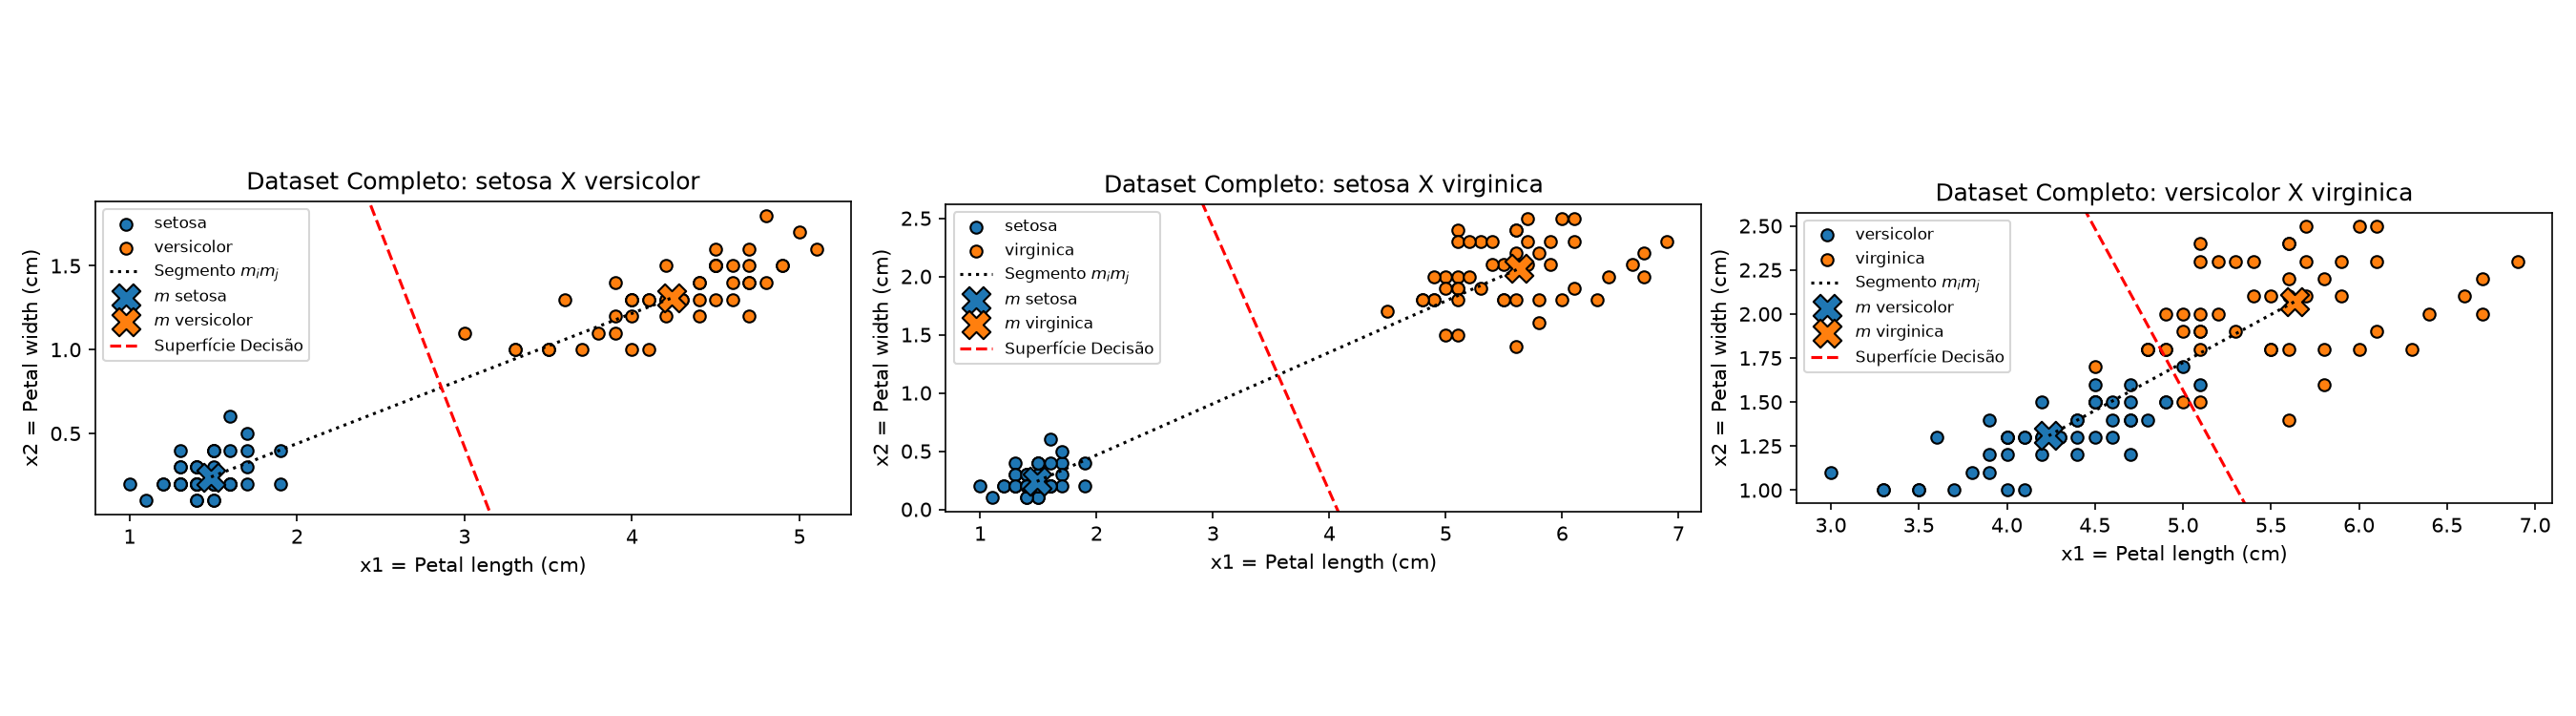
\includegraphics[width=\textwidth]{figuras/superficie_completo.png}
\caption{As mesmas retas, estimadas apenas com o treino, sobre todas as amostras de cada par.}
\label{fig:completo}
\end{figure}

As Figuras~\ref{fig:teste} e~\ref{fig:completo} evidenciam a propriedade geométrica da superfície de decisão do classificador de distância mínima: em todos os cenários a reta tracejada cruza o segmento $\overline{\mathbf{m}_i\mathbf{m}_j}$ no ponto médio e perpendicularmente a ele. Nos pares que envolvem \emph{setosa}, a reta passa pela grande faixa vazia entre as nuvens; no par \emph{versicolor} $\times$ \emph{virginica}, ela atravessa justamente a região de contato, onde se concentram os erros.

%=====================================================================
\section{Discussão}\label{sec:discussao}
%=====================================================================

\paragraph{Equivalência (i) $\equiv$ (ii).} As acurácias e predições idênticas confirmam, na prática, que selecionar a menor distância euclidiana equivale a determinar o máximo da função de decisão. A vantagem da forma (ii) é computacional e conceitual: $d_j(\mathbf{x})$ é \emph{linear} em $\mathbf{x}$ e dispensa a raiz quadrada. Por isso as fronteiras entre classes são retas, o que permite escrevê-las explicitamente, como na Tabela~\ref{tab:retas}.

\paragraph{Coerência entre classificador e superfícies.} Como os três sistemas usam o mesmo vetor de características e os mesmos protótipos, as retas visualizadas são exatamente as fronteiras que o classificador de três classes utiliza: uma amostra é atribuída a $\omega_i$ quando está do lado de $\omega_i$ em todas as retas que envolvem essa classe. Os erros da matriz de confusão (Tabela~\ref{tab:confusao}) correspondem às amostras de teste que aparecem do lado errado da reta \emph{versicolor} $\times$ \emph{virginica} na Figura~\ref{fig:teste}.

\paragraph{Escolha dos atributos.} As dimensões da pétala são as que melhor discriminam as espécies da base Iris. Em uma versão anterior deste trabalho, com a mesma partição dos dados, o classificador que usava os quatro atributos obteve 91,11\% de acurácia no teste, e as retas construídas com as dimensões da sépala acertaram apenas 72\% das amostras no par \emph{versicolor} $\times$ \emph{virginica}, cujas nuvens praticamente se sobrepõem nesse subespaço. Com as duas dimensões da pétala, a acurácia sobe para 93,33\% e a mesma reta chega a 94\%. Isso mostra que acrescentar atributos pouco discriminantes não melhora, e pode até piorar, um classificador de distância mínima, pois todos os atributos pesam igualmente no cálculo da distância.

\paragraph{Limitações do método.} O classificador de distância mínima representa cada classe apenas pela média, ignorando a dispersão e a correlação entre atributos. Na Figura~\ref{fig:variabilidade}, \emph{setosa} forma uma nuvem pequena, enquanto \emph{versicolor} e \emph{virginica} são mais espalhadas e alongadas na direção da reta que une os protótipos; um classificador que levasse em conta essas diferenças de dispersão, como os métodos de máxima verossimilhança e de Bayes, poderia posicionar melhor a fronteira entre essas duas classes.

\paragraph{Avaliação.} Os resultados vêm de uma única partição 70/30 com semente fixa, e o conjunto de teste tem apenas 45 amostras: cada erro equivale a cerca de 2,2 pontos percentuais. Uma estimativa mais robusta exigiria validação (por exemplo, validação cruzada), que, conforme o enunciado, ficará para um momento posterior.

%=====================================================================
\section{Conclusão}
%=====================================================================

Foram implementados, sem bibliotecas de aprendizado de máquina, o classificador de distância mínima, o classificador pelo máximo das funções de decisão e as superfícies de decisão entre pares de classes, todos com o comprimento e a largura da pétala, seguindo fielmente a formulação do reconhecimento por decisão teórica. Os resultados reproduziram as propriedades teóricas do método: (a) os dois classificadores são equivalentes e produziram as mesmas predições, com 93,33\% de acurácia no teste; (b) as superfícies de decisão são bissetores perpendiculares ao segmento entre os protótipos, o que pode ser observado nos gráficos, e a reta \emph{versicolor} $\times$ \emph{setosa} reproduz a do exemplo ilustrativo; e (c) a qualidade da separação depende fortemente dos atributos escolhidos: com a pétala, \emph{setosa} é separada sem erros e \emph{versicolor} e \emph{virginica} são distinguidas em 94\% dos casos, resultado superior ao obtido com a sépala ou com os quatro atributos.
%=====================================================================
% Referências
%=====================================================================
\begin{thebibliography}{9}

\bibitem{sousa}
SOUSA, R. P. de. \textbf{Reconhecimento: base em decisão teórica}. Material de aula da disciplina Tópicos Especiais em Inteligência Artificial. Campina Grande: Universidade Estadual da Paraíba, 2026.

\bibitem{repo}
PAMPLONA, J. \textbf{Laboratório 01: classificador de distância mínima e funções de decisão aplicados à base Iris}. Repositório de código-fonte, 2026. Disponível em: \repositorio. Acesso em: set. 2026.

\end{thebibliography}

\end{document}
